\section{Conclusions}
\subsection{Realistic System Simulation}
\label{subsec:realistic_system_simulation}
Following the analyses described in the previous section, I decided to extend the project with a real graphical simulation, in order to demonstrate that the numerical simulation is correct.\\

\noindent
The parameters used for the real simulation are:

\begin{itemize}
    \item $nstep = 100'000$
    \item $step = 250$
    \item $ni = 100$
    \item $nj = 100$
    \item $tfac = 0.01f$
    \item $size = ni \times nj = 10'000$
\end{itemize}

\begin{figure}[htbp]
    \centering

    % Row 1
    \begin{subfigure}[b]{0.49\textwidth}
        \centering
        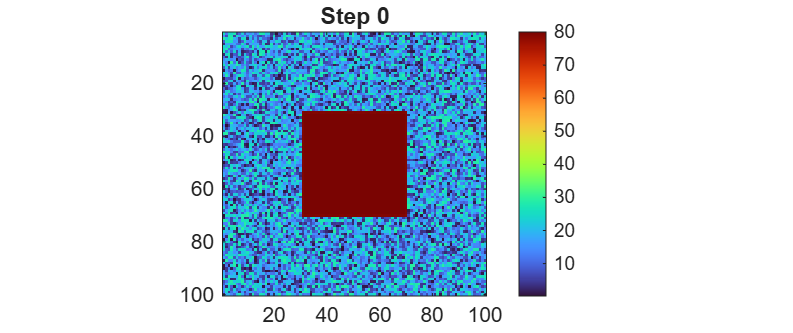
\includegraphics[width=\textwidth]{assets/conclusions/img1.png}
    \end{subfigure}
    \hfill
    \begin{subfigure}[b]{0.49\textwidth}
        \centering
        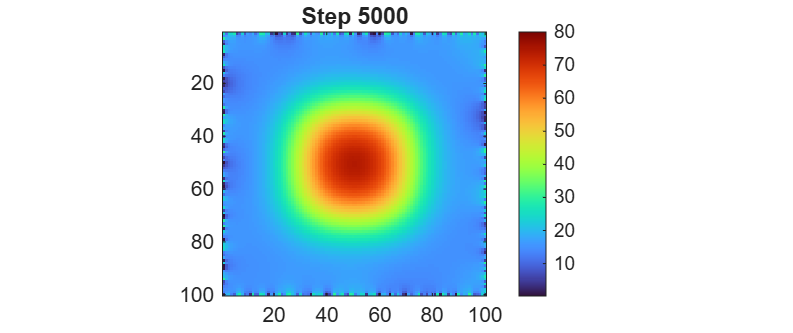
\includegraphics[width=\textwidth]{assets/conclusions/img2.png}
    \end{subfigure}

    \vspace{0.6cm}

    % Row 2
    \begin{subfigure}[b]{0.49\textwidth}
        \centering
        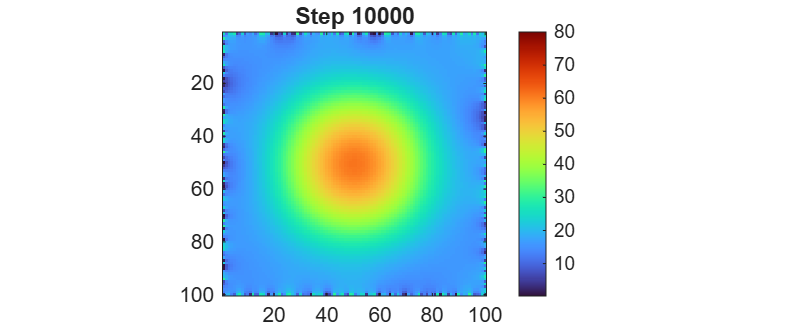
\includegraphics[width=\textwidth]{assets/conclusions/img3.png}
    \end{subfigure}
    \hfill
    \begin{subfigure}[b]{0.49\textwidth}
        \centering
        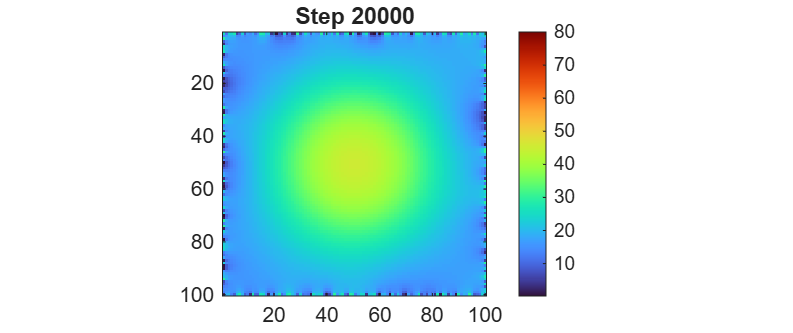
\includegraphics[width=\textwidth]{assets/conclusions/img4.png}
    \end{subfigure}

    \vspace{0.6cm}

    % Row 3
    \begin{subfigure}[b]{0.49\textwidth}
        \centering
        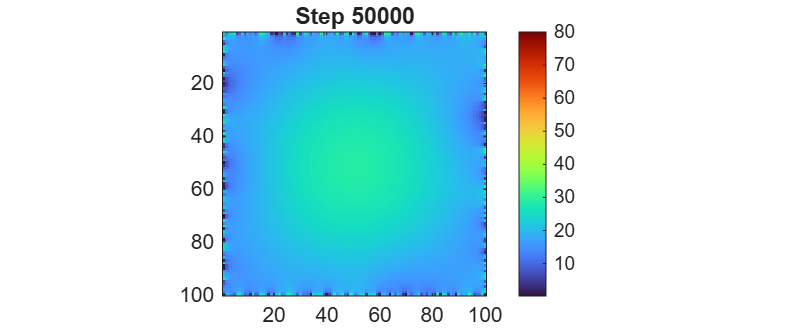
\includegraphics[width=\textwidth]{assets/conclusions/img5.png}
    \end{subfigure}
    \hfill
    \begin{subfigure}[b]{0.49\textwidth}
        \centering
        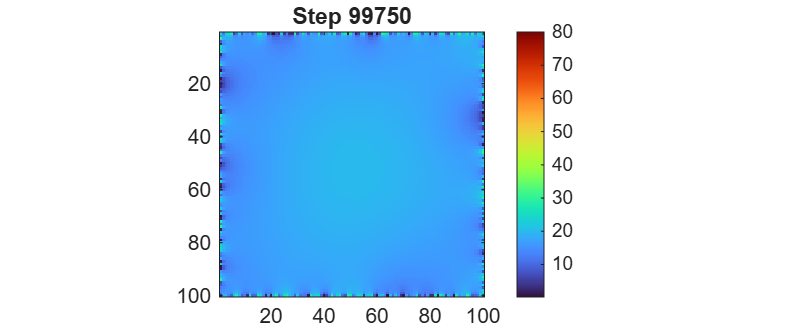
\includegraphics[width=\textwidth]{assets/conclusions/img6.png}
    \end{subfigure}
\end{figure}

\newpage
\subsection{Considerations}
GPU parallelization enabled a significant speedup, demonstrating the effectiveness of this approach compared to the CPU implementation.\\

\noindent
The maximum error between GPU and CPU results was computed to verify correctness. In the current simulation, the maximum observed error remained within acceptable limits (0.0005).\\

\noindent
These results confirm that the CUDA parallelization substantially reduces execution time relative to the sequential version while preserving numerical accuracy